% fix bugs
\RequirePackage{fixltx2e}


\documentclass[10pt]{article}

% encoding of tex-file
\usepackage[utf8x]{inputenc}

% for propper Umlaute
\usepackage[T1]{fontenc}

% proper hyphenation
\usepackage[UKenglish]{babel}

% better i18n Postscript version of Knuth's cm fonts, better than cm-super
\usepackage{lmodern}

% Mathematics
\usepackage{mathtools} % extension and fixes of/in amsmath
\usepackage{amssymb} % provides symbols, loads amsfonts
\usepackage{amsthm} % provides theorem environment
\usepackage{nicefrac} % better slash fracs in inline

% For including figures, rotating or scaling text (dont use file extension)
\usepackage{graphicx}

% own symbol definitions
%
% Math Environements
%
% italic text
\newtheorem{theorem}{Theorem}[chapter]
\newtheorem{corollary}[theorem]{Corollary}
\newtheorem{proposition}[theorem]{Proposition}
\newtheorem{lemma}[theorem]{Lemma}
% normal text
\theoremstyle{definition}
\newtheorem{definition}[theorem]{Definition}
\newtheorem{example}[theorem]{Example}

%
% General Mathematics
%
% natural numbers
\newcommand{\N}{\mathbb{N}}
% real numbers
\newcommand{\R}{\mathbb{R}}
% integer range
\newcommand{\range}[2]{#1,\ldots,#2}
% functions: f\from\R\to\R
\newcommand*{\from}{\colon}
% define as
% FIXME: define "def" properly
%\newcommand{\defeq}{\,\stackrel{\text{def}}{=}\,}
% defined by
\newcommand\logeq{\mathrel{\vcentcolon\Longleftrightarrow}}
% norm
%\DeclarePairedDelimiter{\abs}{\lvert}{\rvert}
\DeclarePairedDelimiter{\nnorm}{\lVert}{\rVert}
\DeclarePairedDelimiter{\supnorm}{\lVert}{\rVert_{\text{\scriptsize{sup}}}}

% exponential function
\newcommand{\e}[1]{\text{e}^{#1}}

%
% Analysis
%
% derivative: Lagrange style
%\newcommand{\D}[1]{#1'} % ' defined in latex and is same as \prime
% derivative: Leibniz style
\renewcommand{\DD}[2]{\frac{\text{d} #1}{\text{d} #2}}
% differential in integral
\newcommand{\dx}[1][x]{\text{d}#1}

\newcommand{\continuouspws}[3][]{\ensuremath{C^{#1}_\text{pw}\ifthenelse{\equal{#2}{}}{}{\ifthenelse{\equal{#3}{}}{(#2)}{(#2,#3)}}}}

%
% Delay Differential Equation
%
% definition domain of right hand side
\newcommand{\deff}{\R\times\R^n\times\R^n}

%
% Differential Dynamic Logic
%
% ddL
\newcommand{\ddL}{\textsf{dd{\kern-0.1em}$\mathcal{L}$ }}
\newcommand{\signature}{\Sigma}
\newcommand{\varsymbols}{V}
\newcommand{\terms}{\lterms{\signature}{\varsymbols}}
\newcommand{\FOLformulas}{\lformulas[\FOL]{\signature}{\varsymbols}}
\newcommand{\FOL}{\text{FOL}}
\newcommand{\FOLR}{\FOL$_\R$}
% FIXME: use \mathcal{M}
\newcommand{\model}{M}
\newcommand{\interpret}[1][]{\ifthenelse{\equal{#1}{}}{I}{I(#1)}}
\newcommand{\universe}{D_{\model}}
\newcommand{\assignment}{\nu}
\newcommand{\ireachability}[2]{\rho\left(#2\right)}
%
% Delay Differential Dynamic Logic
%
\renewcommand{\ivr}{\chi}
\newcommand{\csfml}{\chi}

% formula of first-order real arithmetic
\newcommand{\asfmlfolR}{\chi}

% propositions
\newcommand{\asprop}{p}
\newcommand{\bsprop}{q}

% sets of formulas
\newcommand{\asfmls}{\Gamma}
\newcommand{\bsfmls}{\Delta}
\newcommand{\csfmls}{\Theta}

% states
\newcommand{\states}{\mathcal{S}}
\newcommand{\asstate}{\nu}
\newcommand{\bsstate}{\omega}
\newcommand{\csstate}{\mu}

\newcommand{\delayinterval}[1][T]{[-#1,0]}

\newcommand{\diffvars}{\D{\allvars}}
\newcommand{\delayedvars}{\mathcal{V}_\tau}

\newcommand{\statespace}[1][T]{\continuouspws[0]{\delayinterval[#1]}{\R^n}}
%\newcommand{\xtau}[1][]{\ifthenelse{\equal{#1}{}}{x[\tau]}{x[#1]}}
\newcommand{\x}[1][]{x[#1]}
\newcommand{\xtau}[1][\tau]{x[-#1]}
\newcommand{\Dxtau}[1][\tau]{\D{x}[-#1]}
\newcommand{\holdssince}[3][s]{\lforall{#1\in\delayinterval[#2]}{\left(#3\right)}}

\newcommand{\xbartau}{\bar{x}_{\tau}}
\newcommand{\xbartaut}[1]{\bar{x}_{\tau,#1}}



%%%%%%%%%%%%%%%%%%%%%%%%%%%%%%%%%%%%%%%%%%%%%%%%%%%%%%%%%%%%%%%%%%%%%%%%%%%


\begin{document}

\title{Delay Hybrid Systems}

\author{Lorenz Sahlmann\\ Ecole Polytechnique\\ Carnegie Mellon University}
\date{\today}

\maketitle


In this work we extend Differential Dynamic Logic with Delay Differential Equations.

This requires an extension of the syntax, a (partially) redefinition of the semantics and the introduction of additional axioms and proof rules.

This results in a superset of \dL which we call \textbf{Delay Differential Dynamic Logic}.

\section{Delay Differential Equations}\label{delay-differential-equations}

\subsection{Piecewise Continuous Functions}\label{piecewise-continuous-functions}
The following definition is motivated by capturing the character evolution arising from hybrid systems. We will see that we can consider such to be piecewise continuous.

\begin{definition}[Piecewise Continuous]
    \label{definition-piecewise-continuous}

    Let $D=[a,b]\subset\R$ be a closed interval (this includes the cases when $a=-\infty$ or $b=\infty$, or both). The mapping $x:D\rightarrow\R^n$ is called \textbf{piecewise continuous} if and only if there is a finite subdivision $\{t_i:i=0,\ldots,m\}$ of $D$ (i.e.\ $a=t_0<t_1<\ldots<t_m=b$) such that $x$ is continuous on each interval piece $[t_i,t_{i+1})$ for all $i=0,\ldots,m-1$ and the left sided limits
    \begin{equation}
        \lim_{\substack{t\nearrow t_{i+1}\\ t\in[t_i,t_{i+1})}} x(t)
    \end{equation}
    exist. Hence $x(b)$ can be an isolated point and this right interval limit $b$ is the only spot where such is allowed.

    We denote by $C^0_\text{pw}(D,\R^n)$ the set of \textbf{piecewise continuous functions} on the compact interval $D$ (this excludes the cases with $\pm\infty$), mapping to $\R^n$.

\end{definition}


\begin{figure}[h]\centering
	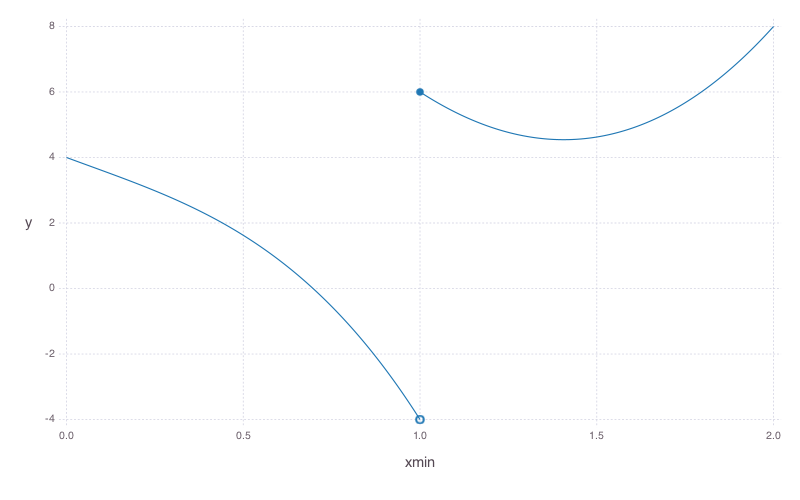
\includegraphics[width=\textwidth]{allowed.png}
	\caption{This figure shows an admissible piecewise continuous function.}
	\label{fig:allowed}
\end{figure}


\begin{figure}[h]\centering
    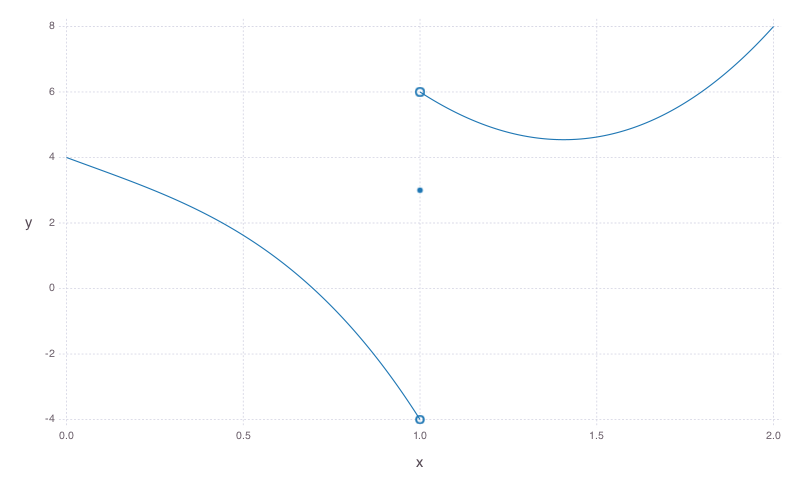
\includegraphics[width=\textwidth]{not-allowed.png}
	\caption{The following function however is not allowed!}
	\label{fig:not-allowed}
\end{figure}

\subsection{Definition DDE}\label{definition-dde}

\begin{definition}[Delay Differential Equation]
    Let $f:\R^n\times\R^n\rightarrow\R^n$ and $\tau > 0$.
    A functional equation of the form
    \begin{equation}
        x'(t) = f\left(x(t),x(t-\tau)\right)
    \end{equation}
    is called \textbf{Delay Differential Equation (DDE)} with \emph{constant, discrete delay}. It is \emph{autonomous}, since its right hand side $f$ is time independent.

    If the right hand side only depends on $x(t-\tau)$ and not on $x(t)$, we call the DDE \emph{pure}.

    A DDE can be equipped with an \textbf{initial condition}. It specifies the values of $x$ on $[-\tau, 0]$ on which the right hand side depends.

\end{definition}

Since we only consider autonomous DDEs, we can without loss of generality restrict to the case of initial time $t_0=0$.

The definition of a DDE can be extended to multiple constant discrete delays. For simplicity, we restrict here to a single delay.

\subsection{Definition of Solution}\label{definition-of-solution}

\begin{definition}[Solution of DDE]
A piecewise continuous function $x\in C^0_\text{pw}([-\tau,T],\R^n)$ is called \textbf{local solution} of the DDE (eq ??), if and only if there exists a $T>0$ such that $x|_{(0,T)}\in C^1((0,T),\R^n)$ with
\begin{equation}
    x'(t) = f\left(x(t),x(t-\tau)\right)
\end{equation}
for all $t\in (0,T)$ and in $t=0$, it holds for the right-hand derivative \begin{equation}
    \lim_{h\searrow 0}\frac{x(h)-x(0)}{h}=f(x(0),x(-\tau))
\end{equation}
and obeys the initial condition:
\begin{equation}
    x(t) = x_0(t) \quad\text{for } t\in [-\tau,0]
\end{equation}
on $[-\tau,0]$.

%TODO: differentiable in right rand point? need not derivative in right hand point

%TODO: Fortsetzbarkeit For example initial condition has jump, this point is limit for local solution.

If the function $x$ is solution for all $T\in\R_{>0}$, it is called \textbf{global}.

\end{definition}

%TODO:
The notion of solution for an autonomous DDE as given above can be lifted to be a trajectory in the statespace
\begin{equation}
    \gamma_x:[0,T]\rightarrow\statespace,\\ t\mapsto\xbartaut{t}
\end{equation}

The \textbf{state} at time $t$ is a function which provides a time limited history up to the current time. This is all information needed to determine (using the DDE) to determine the solution for time $\geq t$. It is defined as $\xbartaut{t}(s)\defeq x(t+s)$ for $s\in [-\tau,0]$. In the case of $t=0$, we simplify the notation to $\xbartau \defeq \xbartaut{0}$.

This notion of solution is a \emph{dynamical systems} point of view which later turns out to be useful.

\paragraph{Lemma}\label{lemma}

%TODO: solving dde equiv to solving integral equation??? (-\textgreater{} Lemma) and compare with ODE lecture notes

Finding a solution of the DDE (??) is equivalent to computing the integral

\begin{equation}
    x(t) = x_0(0) + \int_0^t g(\bar{x}_{\tau,s})ds
\end{equation}

\paragraph{Proof}\label{proof}

integrate from discontinuity of $\xbartaut{t}$ to discontinuity and proof stetige fortsetzbarkeit at these points

\subsection{Method of Steps}\label{method-of-steps}
for $t\in [0,\tau]$, $x$ must satisfy the following ordinary initial value problem obtained by plugging the initial function into equation (??). For suitable $f$ and $x_0$, the existence (and uniqueness) of a solution on $[0,\tau]$ is guaranteed by ODE theory (\ldots{} or Picard-Lindelöf theorems).

This procedure can then be applied repeatedly to extend the obtained solution by steps of length $\tau$.

\subsection{Existence and Uniqueness of Solutions}\label{existence-and-uniqueness-of-solutions}

$f$ Lipschitz with piecewise continuous initial function have existence and uniqueness ???? smoothing

\paragraph{Theorem}\label{theorem}
Consider the autonomous Delay Differential Equation

%TODO: do we need global existence or just local?

%TODO: this DDE is more general than in definition above

\begin{equation}
    \begin{cases}
        x'=f(\xbartaut{t}) & \text{for } t\geq 0\\
        x(t)=x_0(t)     & \text{for } t\in [-\tau,0]
    \end{cases}
\end{equation}

with $f:\statespace\rightarrow\R^n$ satisfying the (local) Lipschitz condition
\begin{equation}
    \forall M>0\,\exists L>0\,\forall x,y\in C^0([-\tau,0],\R^n) : \norm{x},\norm{y}\leq M\Rightarrow\abs{f(x)-f(y)} \leq L\norm{x-y}
\end{equation}
where $\abs{\cdot}$ denotes the Euclidian norm on $\R^n$ and $\norm{\cdot}$ the supremum norm of the Banach space of continuous functions on $[-\tau,0]$.

Then for each \textbf{bounded initial condition} $x_0\in\statespace$, i.e.\ $\norm{x_0}< \infty$, there \textbf{exists} a \textbf{unique local solution} of the DDE on a time interval $[-\tau, T]$ with $T>0$.

\paragraph{Proof}\label{proof-1}
use Theorem 3.7 from {[}{]} or \ldots{}

just proof existence/uniqueness on each peace of continuity proof continuity at knots with Lemma of integral equ

\paragraph{Corollary}\label{corollary}
when f is polynomial and depends on $x(t)$ and $x(t-\tau)$ then theorem holds

polynomial -\textgreater{} continuously differentiable -\textgreater{} locally Lipschitz

%TODO: can write DDE (eq??) from definition as

\begin{equation}
    \begin{cases}
        x'=f(\xbartaut{t})\defeq g(\xbartaut{t}(0),\xbartaut{t}(-\tau)) &\text{for } t\geq 0\\
        x(t)=x_0(t) & \text{for } t\in[-\tau,0]
    \end{cases}
\end{equation}

\paragraph{Proof}\label{proof-2}

\subsection{Example}\label{example}
The basic ODE IVP
\begin{equation}
    \begin{cases}
        x'(t) = -x(t)\\
        x(0) = x_0
    \end{cases}
\end{equation}
has the solution $x(t)=x_0 e^{-t}$. However the similiar DDE
\begin{equation}
    \begin{cases}
        x'(t) = -x(t-\tau) & t\geq 0\\
        x(t) = x_0(t) & -\tau\leq t\leq 0
    \end{cases}
\end{equation}
has a much richer dynamics, but solution (as series) for $x_0\equiv 1$, can compute first solutions by method of steps. \ldots{}

\begin{figure}[h]\centering
    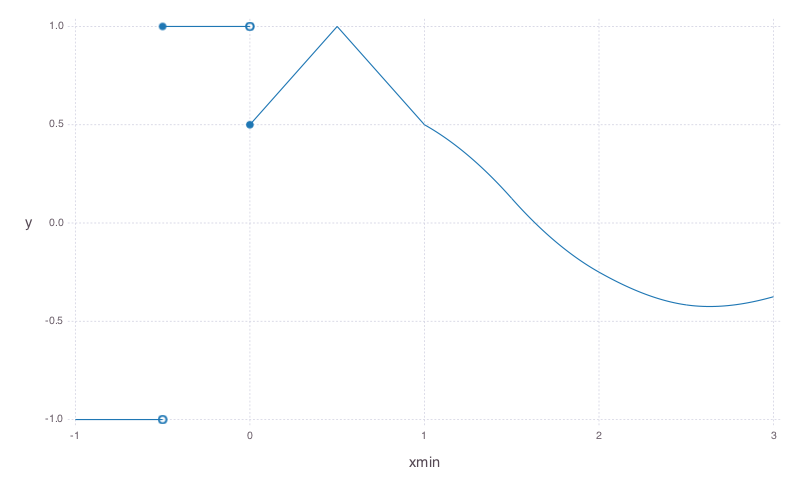
\includegraphics[width=\textwidth]{piecewise-initial-function.png}
	%\caption{}
	\label{fig:not-allowed}
\end{figure}

\subsection{Definition}\label{definition}

\section{Hybrid Programs with DDEs}\label{hybrid-programs-with-ddes}

Extent classic hybrid programs (HP) with syntax, semantics and axiomatization and proof rules for DDEs. Is a super set, \dL is a fragment

\subsection{Example}\label{example-1}

leading and following car

\subsection{Syntax}\label{syntax}

\paragraph{Terms}\label{terms}

We extent the grammar defining \textbf{terms} with a symbol for a \textbf{delayed variable}

\begin{equation} \theta,\eta := x|\xtau|c|\theta+\eta|\theta\cdot\eta \end{equation}

\subsection{Semantics}\label{semantics}

HP $\alpha$ transition semantics define inductively

remain unchanged

The temporal character of delay differential equations (they depend on their own temporal evolution with limited horizon) suggests the introduction of trace semantics.

However, we go the way of introducing transition semantics with an augmented state space.

\paragraph{Terms}\label{terms-1}

Following the remark to the solution of a DDE, we change the \textbf{state space} to $\statespace$, the set of piecewise continuous functions, as defined above.

%TODO: need $\xbartau$

Denote by $\states$ the set of states. A state $\omega\in\states$ is a mapping $\omega : \mathcal{V}\cup\mathcal{V'}\rightarrow\statespace$ that assigns a \emph{history} (function) $\xbartau$ to each variable symbol and
%FIXME: diff var symbol.

The semantics of the variable symbols in terms are given by
\begin{equation}
    [[\xtau]]_\nu=\nu(x)(-\tau)\defeq:\xbartau(-\tau)
\end{equation}
and
\begin{equation}
    [[x]]_\nu=\nu(x)(0)\defeq:\xbartau(0)
\end{equation}

When we write $\xtau$ we mean $x(t-\tau)$ and with $x$ we mean $x(t)$.

\paragraph{Hybrid Programs}\label{hybrid-programs}

The transition semantic of a hybrid program is inductively given by a binary reachability relation $\rho(\alpha)\subseteq\states\times\states$. Since the state space has been replaced, we need to redefine the semantics:

The \emph{discrete assignment} does not rewrite history, but changes only the value at the current time instant:
\begin{equation}
\rho(x:=\theta) = \left\{(\nu,\omega): \omega = \nu \text{ except } \omega(x)=\left(t\mapsto\begin{cases}[[\theta]]_\nu & t=0\\ \nu(t) &t\in[-\tau,0)\end{cases}\right)\qquad\right\}_.
\end{equation}
This assignment is the actual reason why we need to consider piecewise continuous evolutions.

%TODO: super dense time: multiple assignments

Using the extended syntax, we can write down both a delay differential equation and an ordinary differential equation in the form $x'=\theta$, where $\theta=f(x,\xtau)$ with a polynomial $f$.

\begin{equation}
    \rho(x'=\theta\,\&\,\chi) = \left\{ (\varphi(0),\varphi(s))\,:\,\varphi(t)\models x'=\theta\,\wedge\,\varphi(t)\models\chi\,\forall\,0\leq t\leq s\text{ for a solution } \varphi:[0,s]\rightarrow\states \right\}
\end{equation} As a solution, $\varphi$ needs to fulfill \begin{equation}
    \varphi(t)(x')(0) \defeq \DD{\varphi(\zeta)(x)(0)}{\zeta}(t) \stackrel{!}{=} [[\theta]]_{\varphi(t)(x)}
\end{equation}

\section{Delay Differential Dynamic Logic}\label{delay-differential-dynamic-logic}

\dL terms

\subsection{Dynamic Axioms}\label{dynamic-axioms}

\paragraph{History Axiom}\label{history-axiom}
The occurence of $\xbartau$ in expressions can be replaced by turning the (implicitely existing) time variable explicit, i.e.\
\begin{equation}
    F(\xbartau) \leftrightarrow \forall\,-\tau\leq t\leq 0\, F(x(t))
\end{equation}

\paragraph{Axiom of Steps}
\label{axiom-of-steps}
The \emph{Method of Steps} presented above translates into an axiom. It allows to partially unwind an autonomous DDE given a analytic representation of its solution.

Let $\theta_0$ and $\theta$ be %TODO: \ldots{}
\begin{equation}
    \xbartau = \theta_0 \rightarrow [x'=\theta(\xbartaut{t})]\phi
    \leftrightarrow
    \left(\forall 0\leq t\leq\tau: [x:= y(t)]\phi \right)
    \wedge \xbartaut{\tau} = y \rightarrow [x'=\theta (\xbartaut{t})]\phi
\end{equation} where $\forall 0\leq t\leq\tau$, $y'(t)=\theta(\theta_0)$,
i.e.\ $y$ is a local solution of the DDE. The solution must be expressible in polynomial form so that the axiom leads to decidable arithmetic.

(Since the DDE is autonomous, we can emit the time index.)

\paragraph{Proof}\label{proof-3}
apply methods of steps

\subsection{Proof Rules}\label{proof-rules}

\paragraph{Rule of Steps}\label{rule-of-steps}

condition valid for initial condition and given condition for a $s\leq t$ then condition holds after dde-evolution of max time tau and safety follows from condition then condition holds after dde with mentioned initial condition
\begin{equation}
\frac{\Gamma(\xbartaut{0})\rightarrow F(\xbartaut{0})\quad F(\xbartaut{s})\rightarrow [x'=\theta(\xbartaut{t})\,\&\,t\leq\tau]F(\xbartaut{t}) \quad F(\xbartaut{t})\rightarrow\phi}{\Gamma(\xbartaut{0}) \rightarrow [x'=\theta(\xbartaut{t})]\phi}
\end{equation}

\paragraph{Delay Differential Invariant}
\label{delay-differential-invariant}

Usually, one would try not to mention $\xtau$ in the invariant, since derivation would lead to the occurrence of the symbol $x_{2\tau}$, whose properties are out of the scope of the current state.

%TODO: much doubt if that is sound
\begin{equation}
    \frac{H\wedge\forall\,t-\tau\leq s<t: F(x(s))\rightarrow (F')^{\theta}_{x'}}{F(\xbartau)\rightarrow [x'=\theta(\xbartaut{t})\,\&\,(H\wedge t\leq\tau)]F(\xbartaut{t})}
\end{equation}

\subsection{Example}
\label{example-2}
We want to proof the safety condition $\phi\equiv(-1\leq x\wedge x\leq 1)$ for the continuous program with delay differential equation
\begin{equation}
    \forall\,t\in[-\tau,0]:\,-1\leq\xbartaut{0}(t)\wedge\xbartaut{0}(t)\leq 1
    \rightarrow
    [x'=-\xtau] (\forall\,s\in[-\tau,0]:\,-1\leq\xbartaut{t}(s)\wedge\xbartaut{t}(s)\leq 1)
\end{equation}
in explicit quantified representation. It can be simplified by using an implicit time variable and a context depending meaning of $\xtau$
\begin{equation}
    -1\leq\xtau\leq 1 \rightarrow [x'=-\xtau]\phi.
\end{equation}

We apply the rule of steps using the safety condition $\phi$ as step condition $F(x)\equiv(\forall\,t\in[-\tau,0]:\,-1\leq x(t)\wedge x(t)\leq 1)$.

The first and third premisses hold. The second by ??? (delay differential invariant)

Use the algebraic differential invariant $F\equiv(-1\leq x^3\wedge x^3\leq1)$, which is valid for the initial condition. Differentiation leads to the inequalities, which needs to be shown $\forall t\in[0,\tau]$
\begin{equation}
    0\leq 3\,x(t)^2 x'(t) = -3\,x(t)^2 \xtau(t)
\end{equation}

This holds since


\end{document}
